\subsection*{2.2 Elektrischer Fluss $\Psi$}
    \begin{minipage}{0.49\linewidth}
        \mathbox{
            \Psi = \int \vec{E} d \vec{A}
        }
    \end{minipage}
    \begin{minipage}{0.49\linewidth}
        \begin{scriptsize}
            $E$ = Elektrisches Feld\\
            $A$ = Fläche, durch die das Feld hindurchfliesst
        \end{scriptsize}
    \end{minipage}

    \begin{minipage}{0.54\linewidth}
        \begin{empheq}[box = \fbox]{align*}
            \oint \vec{E} \vec{dA} = \frac{1}{\varepsilon_0} \int \rho dV = \frac{Q}{\varepsilon_0}\\
            div(\vec{E}) = \frac{1}{\varepsilon_0} \rho
        \end{empheq}
    \end{minipage}
    \begin{minipage}{0.44\linewidth}
        \begin{scriptsize}
            Mittels dem Satz von Gauss erhält man die erste Maxwell Gleichung\\
            $\rho$ = Ladungsdichte\\
            $Q$ = Gesamtladung innerhalb der Fläche
        \end{scriptsize}
    \end{minipage}

    \subsubsection{Elektrisches Feld Kugel / Punktladung}
        \begin{minipage}{0.59\linewidth}
            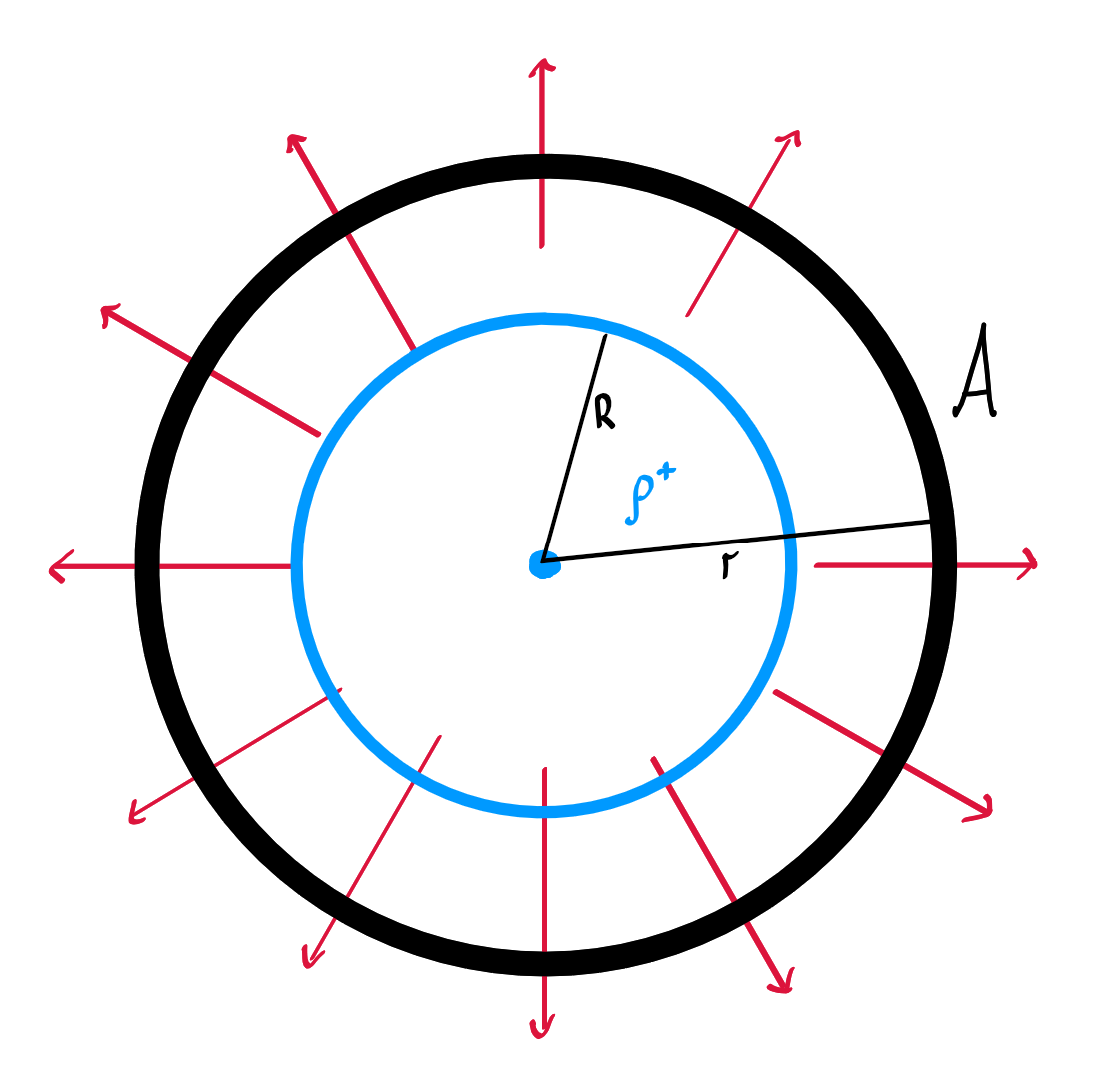
\includegraphics[width = \linewidth]{src/images/e-feld_punktladung.png}
        \end{minipage}
        \begin{minipage}{0.39\linewidth}
            \begin{empheq}{align*}
                \oint \vec{E} \vec{dA} &= \frac{1}{\varepsilon_0} \int \rho dV\\
                \rho&= \frac{Q}{V} = \frac{3Q}{4 \pi R^3}
            \end{empheq}
        \end{minipage}
        \[\begin{array}{c | c}
            r < R & r \geq R\\
            \hline \hline
            \Rightarrow E \cdot 4 \pi r^2 = \frac{\rho \cdot \frac{4}{3} \pi r^3}{\varepsilon_0} & \Rightarrow E \cdot 4 \pi r^2 = \frac{\rho \cdot \frac{4}{3}\pi R^3}{\varepsilon_0}\\
            \Rightarrow E = \frac{\rho r}{3 \varepsilon_0} = \frac{1}{4 \varepsilon_0 \pi } \frac{Q r}{R^3} & \Rightarrow E = \frac{\rho R^3}{3 \varepsilon_0 r^2} = \frac{1}{4 \varepsilon_0 \pi} \frac{Q}{r^2}
        \end{array}\]

    \subsubsection{Elektrisches Feld gerader Leiter}
        \begin{minipage}{0.39\linewidth}
            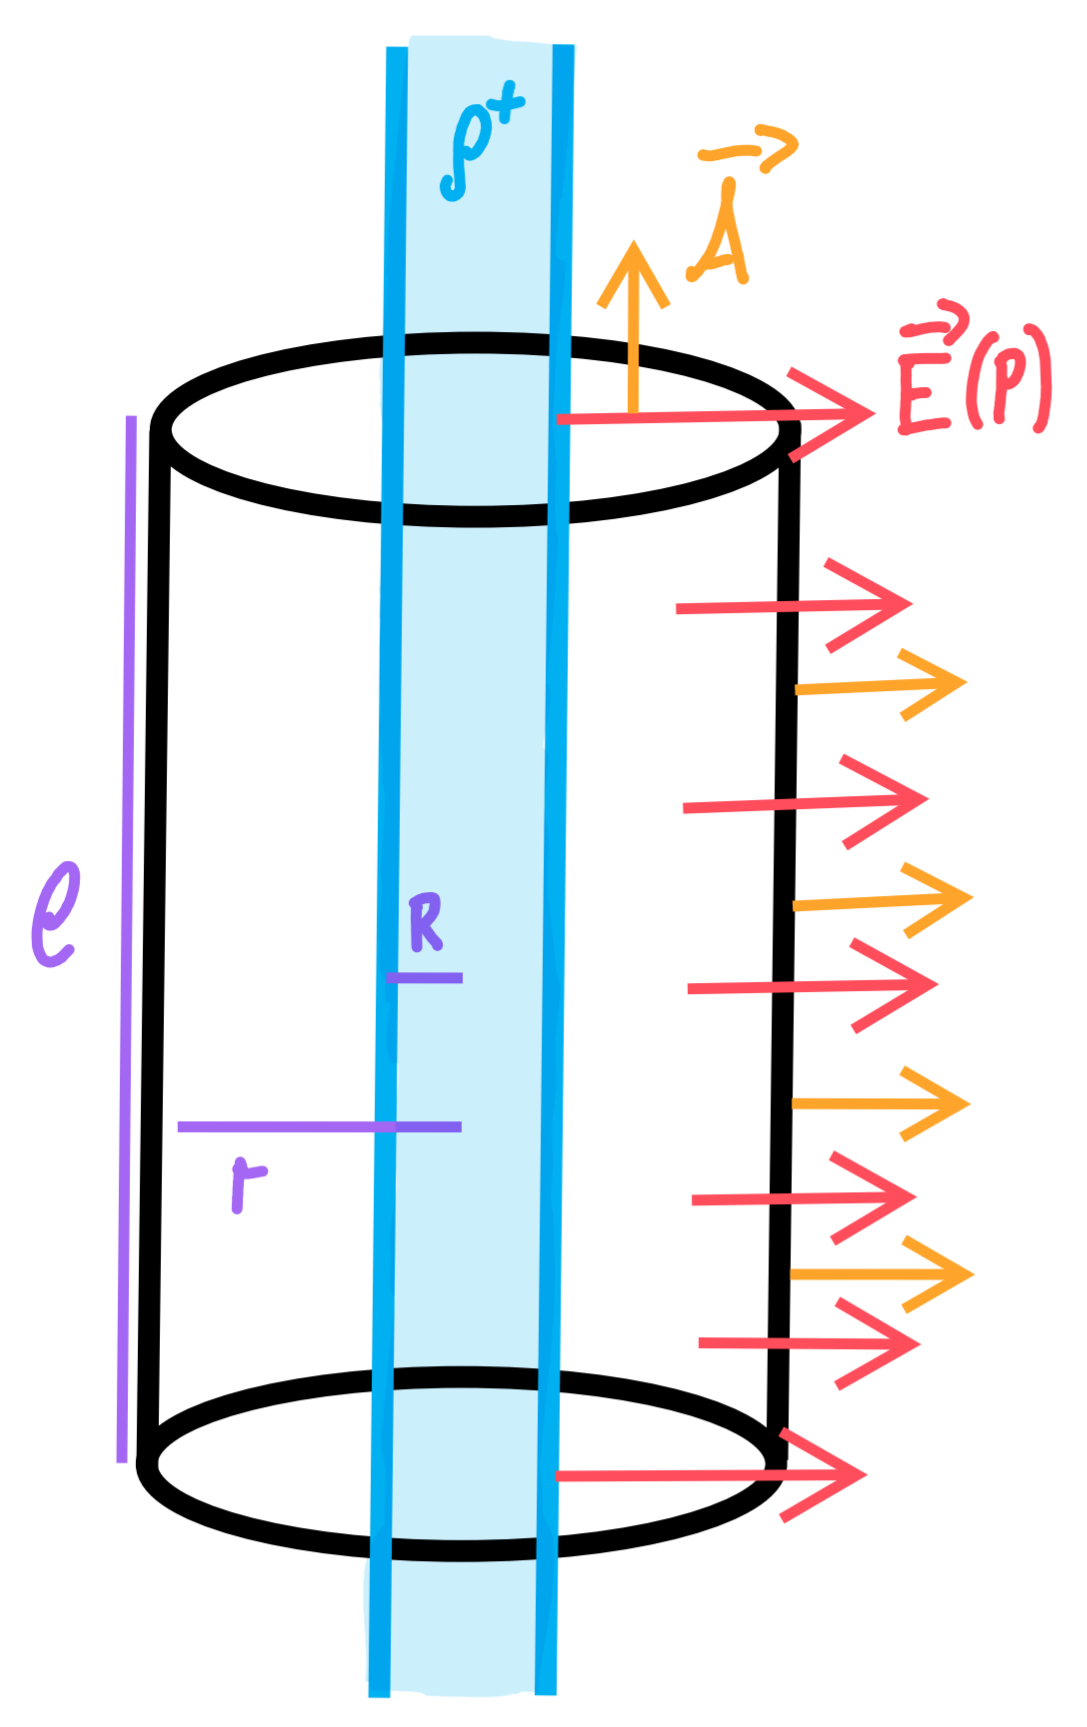
\includegraphics[width = \linewidth]{src/images/e-feld_gerader_leiter.png}
        \end{minipage}
        \begin{minipage}{0.59\linewidth}
            \begin{empheq}{align*}
                \oint \vec{E} \vec{dA} &= \frac{1}{\varepsilon_0} \int \rho dV\\
                \rho &= \frac{Q}{V} = \frac{3Q}{4 \pi R^3}\\
            \end{empheq}
        \end{minipage}
        \[\begin{array}{c | c}
            r < R & r \geq R\\
            \hline \hline
            E \cdot 2 \pi r \cdot l = \frac{\rho}{\varepsilon_0} \pi r^2 l & E \cdot 2 \pi r \cdot l = \frac{\rho}{\varepsilon_0} \pi R^2 l\\
            E = \frac{\rho}{2 \varepsilon_0} r & E = \frac{\rho}{2 \varepsilon_0} \frac{R^2}{r}
        \end{array}\]

    \subsubsection{Elektrisches Feld Platte}
        \begin{minipage}{0.49\linewidth}
            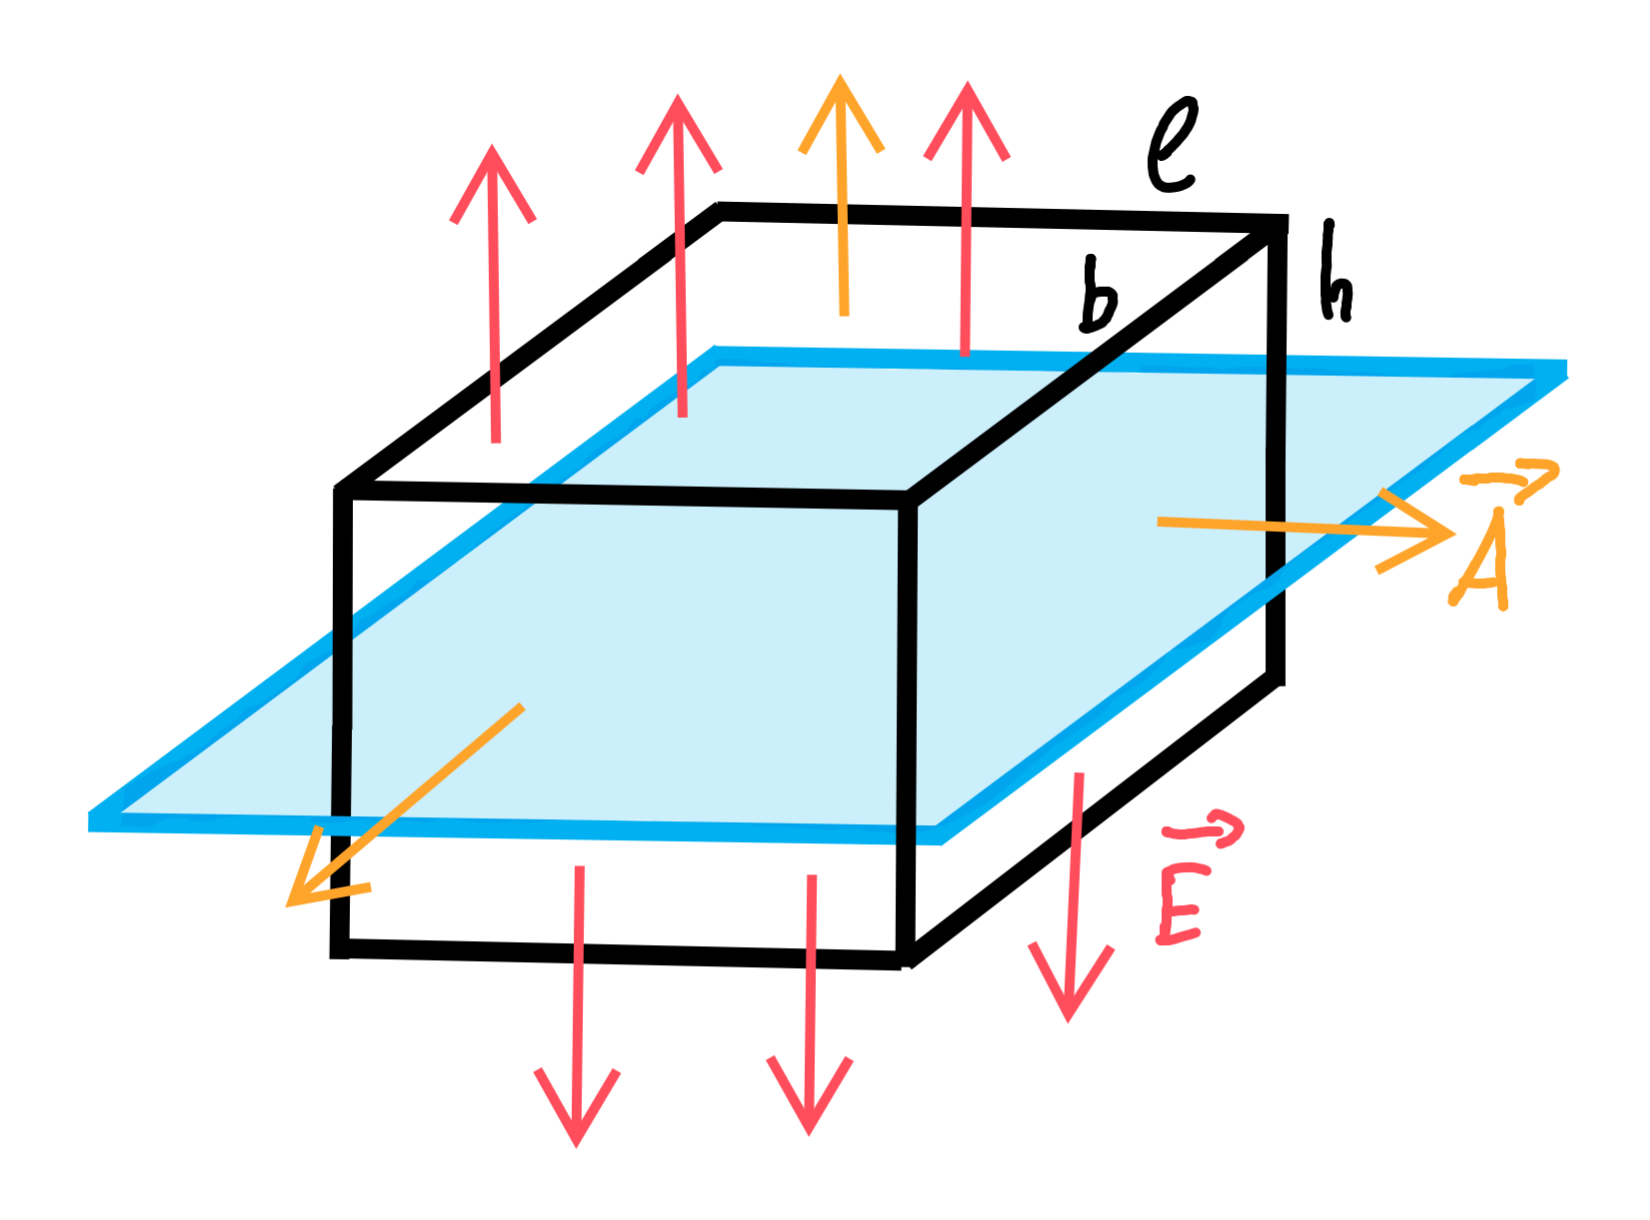
\includegraphics[width = \linewidth]{src/images/e-feld_platte.png}
        \end{minipage}
        \begin{minipage}{0.49\linewidth}
            \begin{empheq}{align*}
                &\oint \vec{E} \vec{dA} = \frac{1}{\varepsilon_0} \int \rho dV\\
                &\rho = \frac{Q}{A} = \frac{Q}{l \cdot b}\\
                \Rightarrow &E \cdot 2 l \cdot b = \frac{1}{\varepsilon_0} l \cdot \rho\\
                \Aboxed{\Rightarrow &E = \frac{\rho}{2 \varepsilon_0}}
            \end{empheq}
        \end{minipage}